\vspace{-1cm}
\begin{wrapfigure}[11]{r}{5.5cm}
  \centering
  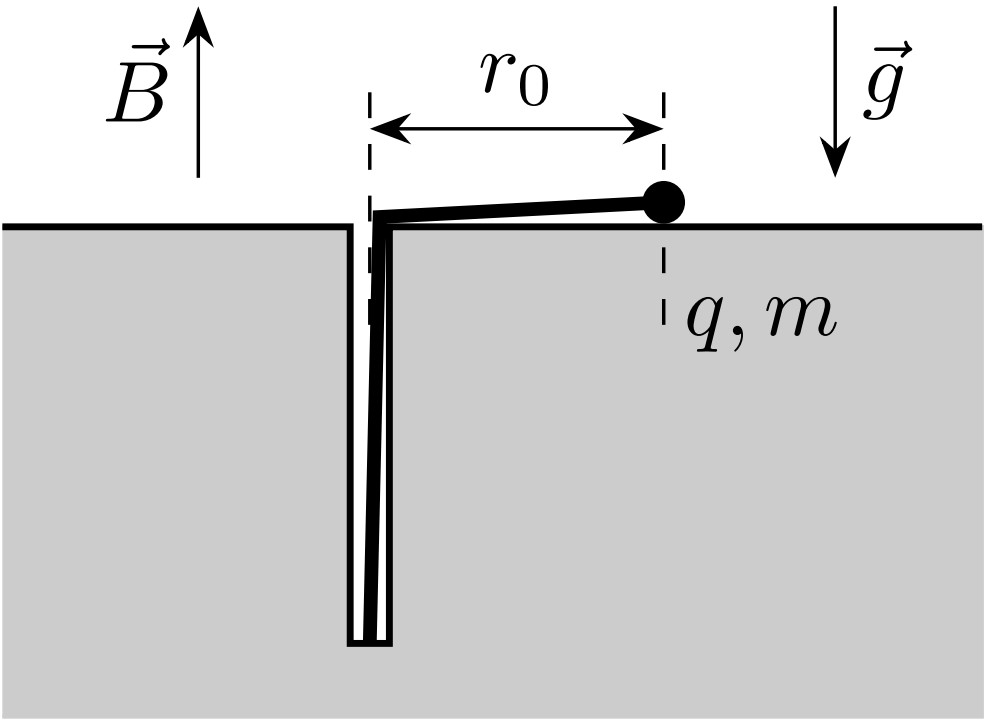
\includegraphics[width=0.3\textwidth]{Figures/Fig 1.jpg}
  \begin{center}
    \figurename{ 1}
  \end{center}
\end{wrapfigure}

\noindent Cho một tấm được làm từ vật liệu không dẫn điện có khoan một lỗ nhỏ thẳng đứng theo hướng vuông góc với bề mặt của tấm, độ sâu của lỗ nhỏ hơn độ dày của tấm. Một đầu của một sợi dây cao su có hệ số đàn hồi $k$ được gắn cố định vào đáy lỗ. Chiều dài tự nhiên của dây cao su bằng với độ sâu của lỗ. Đầu còn lại của sợi dây được gắn với một viên bi có khối lượng $m$ và điện tích $q$. Tấm được đặt nằm ngang trong trọng trường $\vec{g}$ và bề mặt của tấm là nhẵn. Một từ trường đồng nhất có vector cảm ứng từ $\vec{B}$ ngược hướng với gia tốc trọng trường $\vec{g}$ được thiết lập. Ban đầu, viên bi nằm tại vị trí cách lỗ một khoảng $r_{0}$ sau đó được thả ra với vận tốc có phương vuông góc với dây cao su sao cho viên bi chuyển động trên một đường tròn.
\begin{enumerate}
  \item Xác định vận tốc góc của viên bi khi nó chuyển động theo chiều kim đồng hồ và ngược chiều kim đồng hồ (nhìn từ trên xuống).
\end{enumerate}
\noindent Lực tác dụng lên viên bi thay đổi tuyến tính theo vector vị trí $\vec{r}$ và vận tốc $\vec{v}$ của viên bi. Do đó, nếu ta tìm được hai phương trình chuyển động khác nhau $\vec{r}_{1}(t)$ và $\vec{r}_{2}(t)$ mô tả chuyển động của viên bi dưới tác dụng của một lực có đặc tính nêu trên thì phương trình $\vec{r}(t)=\alpha\vec{r}_{1}(t)+\beta\vec{r}_{2}(t)$, với $\alpha$ và $\beta$ là các hằng số, cũng sẽ mô tả một chuyển động khả dĩ của viên bi dưới tác dụng của một lực tương tự. Ví dụ, nếu ta thả viên bi từ cùng một vị trí ban đầu như ở ý 1 mà với vận tốc đầu bằng không thì chuyển động của nó có thể xem như là chồng chập của các chuyển động tròn đã được khảo sát ở ý trên.

\begin{enumerate}
  \setcounter{enumi}{1}
  \item Xác định khoảng cách ngắn nhất của viên bi so với lỗ nếu viên bị được thả ra với vận tốc ban đầu bằng không tại vị trí cách lỗ một khoảng $r_{0}$.
  \item Sau bao lâu kể từ khi thả, viên bi lại cách lỗ một khoảng $r_{0}$?
  \item Trong trường hợp $q^{2}B^{2}/mk=1/2$, sau bao lâu kể từ khi được thả, viên bi sẽ quay lại vị trí ban đầu lần đầu tiên? Phác hoạ quỹ đạo của viên bi trong trường hợp này.
\end{enumerate}
